% AI651 Assignment 2 report.
% Build from this folder: pdflatex main.tex (run twice), or upload the
% report/, q1/ and Question2/ folders to Overleaf and compile report/main.tex.
\documentclass[11pt,a4paper]{article}

\usepackage[margin=2cm]{geometry}
\usepackage[T1]{fontenc}
\usepackage{lmodern}
\usepackage{amsmath,amssymb}
\usepackage{graphicx}
\usepackage{array}
\usepackage{longtable}
\usepackage{booktabs}
\usepackage{enumitem}
\usepackage{caption}
\usepackage{subcaption}
\usepackage{float}
\usepackage[hidelinks]{hyperref}

\graphicspath{{../q1/}{../Question2/figures/}}
\setlist{nosep,leftmargin=1.5em}
\setlength{\parindent}{0pt}
\setlength{\parskip}{4pt}
\renewcommand{\arraystretch}{1.25}
\newcolumntype{L}[1]{>{\raggedright\arraybackslash}p{#1}}

\begin{document}

\begin{center}
  {\Large\bfseries AI651 -- Deep Learning for Space, Time and Graphs}\\[2pt]
  {\large Assignment 2}\\[6pt]
  Name: \textbf{Imran Saeed} \qquad Roll number: \textbf{25280083}\\
  GitHub repository (public): \url{https://github.com/Imran-TheProgrammer/space-time-forecasting-convlstm-and-attention}
\end{center}
\hrule
\vspace{6pt}

% =====================================================================
\section*{Question 1 -- River Forecasting Proposal}

\textbf{Summary of the design.} Every 10 minutes we build a 24-hour history for 8 places: the reservoir, S1, T1, S2, S3, S4, R1 and R2. A small time encoder cleans each place's history. Then one attention step lets each station look at its own past, all places upstream of it, the rain gauges and the announced future releases, \emph{at any time lag}. A small head per station predicts the change in water level over the next hour, as three quantiles (10\%, 50\%, 90\%).

% ---------------------------------------------------------------------
\subsection*{1. Architecture diagram}

\begin{figure}[h]
  \centering
  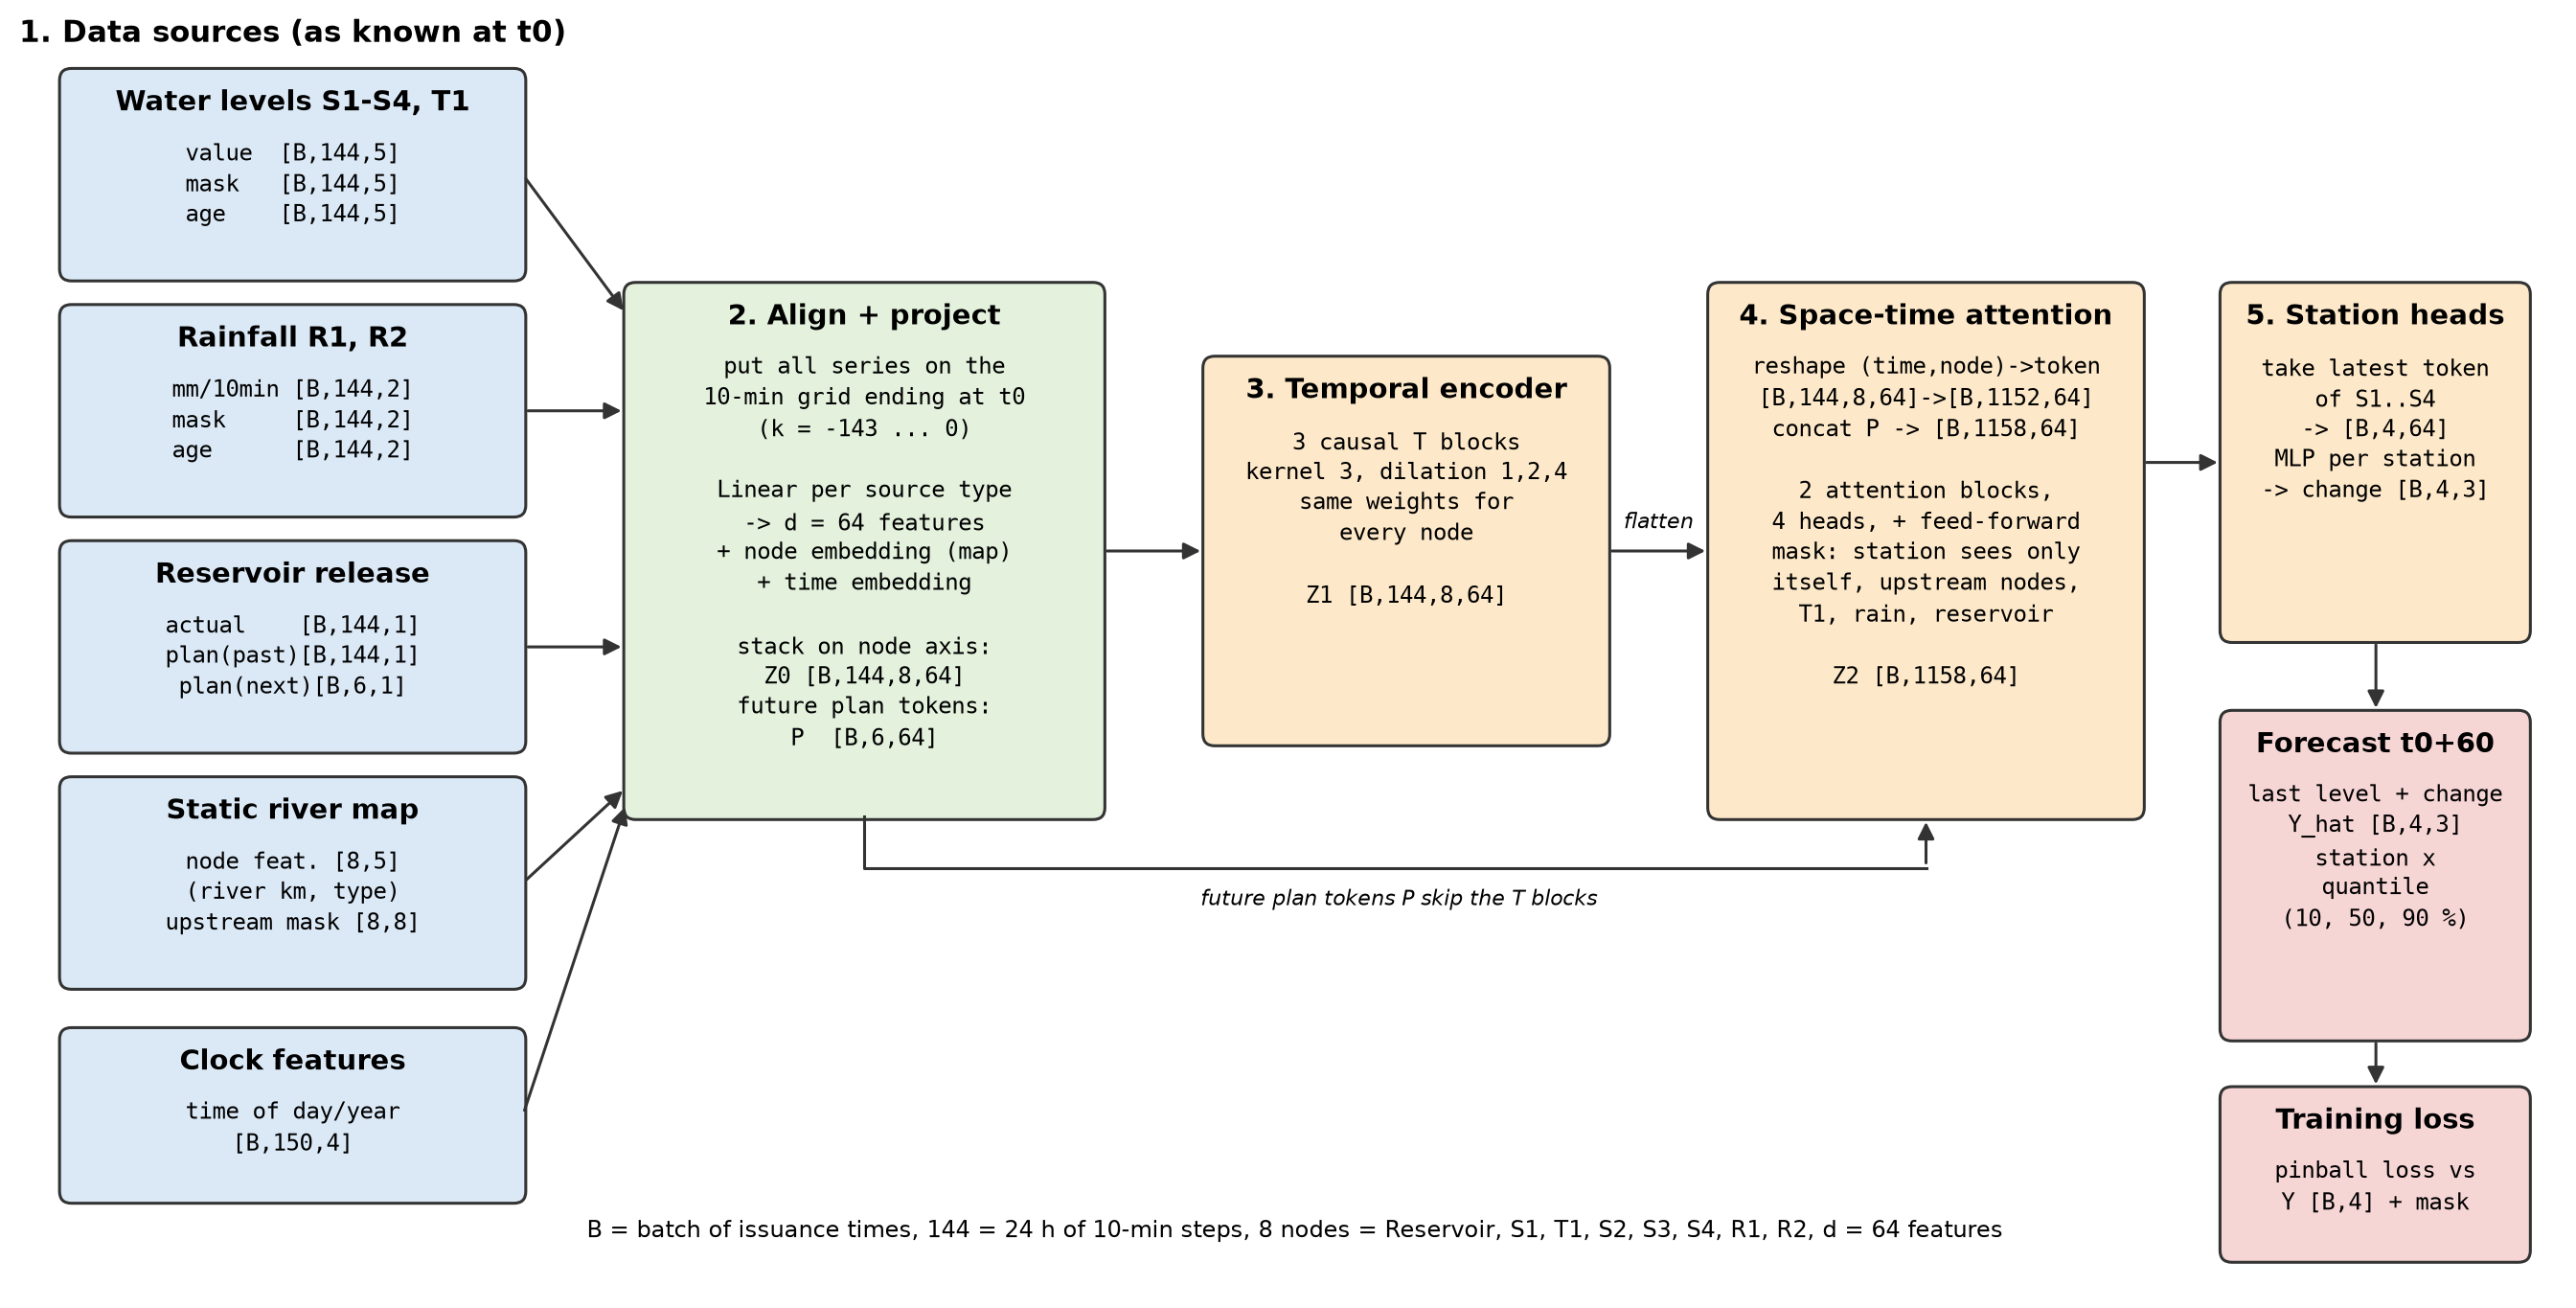
\includegraphics[width=\textwidth]{architecture.png}
  \caption*{\textbf{Q1 architecture.} $B$ = batch of issuance times. 144 = 24 h of 10-minute steps. Node order: Reservoir, S1, T1, S2, S3, S4, R1, R2. All inputs use only data that has arrived by the issuance time $t_0$.}
\end{figure}

\textbf{Joining the sources.} (1) Every series is put on one 10-minute grid that ends at $t_0$. (2) Each source type has its own linear layer that maps its features to the same size $d=64$. (3) The results are stacked on a node axis: $[B,144,8,64]$. (4) Before attention, the time and node axes are flattened into one token axis: $[B,1152,64]$. The 6 future release tokens are added at the end: $[B,1158,64]$. (5) The heads read the token at time $t_0$ for S1--S4: $[B,4,64]$.

% ---------------------------------------------------------------------
\subsection*{2. Assumptions}

\textbf{Supplied facts (not assumptions):} levels at S1--S4 and T1 every 10 min; rain at R1 and R2 with timestamps and locations; recorded releases and announced schedules with announcement and effective times; station locations, river connections and distances; no data on the unmonitored tributary; no future rain or future levels at issuance.

\begin{longtable}{|L{0.6cm}|L{8cm}|L{7.4cm}|}
\hline
\textbf{No.} & \textbf{Assumption and why it is reasonable} & \textbf{Effect on the design} \\ \hline
\endhead
A1 & All clocks use one time zone (UTC), and each level timestamp marks the end of its 10-minute interval. This is normal for a single authority's network. & Readings are placed on the grid by timestamp, with no shifting. \\ \hline
A2 & Level readings usually arrive within 10--20 minutes, but sometimes much later. The arrival time of each reading is logged. & We add an ``age'' input. Training uses only data that had arrived by each past $t_0$ (``as-of'' data). \\ \hline
A3 & Rain gauges report at uneven times (for example tipping buckets). & Rain is summed into 10-minute totals on the same grid. \\ \hline
A4 & The record covers at least 3--5 years at 10-minute steps, including several floods. & This is enough data to learn travel times and rain response. Train, validation and test are split by whole time periods, not at random. \\ \hline
A5 & Level sensors have small noise (about 1 cm) and sometimes spikes or flat lines. The authority flags known bad data. & Flagged or impossible values are treated as missing. \\ \hline
A6 & Each gauge's zero point is fixed, or the authority gives the offsets when it changes. & Levels can be compared across years. Each station is scaled by its own mean and spread. \\ \hline
A7 & No backwater: within one hour, a downstream level does not push an upstream level up. & A station may only attend to itself, nodes upstream of it, the rain gauges and the reservoir. \\ \hline
A8 & Travel time from the reservoir to S4 is under 12 hours at all flows. It is shorter at high flow. & A 24-hour history window covers every travel time with margin. Attention picks the lag, so no fixed lag is assumed. \\ \hline
A9 & R2 lies close to the catchment of the unmonitored tributary (as in the picture). & R2 rain acts as a stand-in for the unmonitored inflow into S3 and S4. \\ \hline
A10 & Release schedules are normally announced at least one hour before they take effect. A newer announcement replaces older ones. Emergency changes can come with less notice. & The planned release for $t_0+10$ to $t_0+60$ min is a known future input. \\ \hline
A11 & Recorded actual releases arrive within 10 minutes. & Past actual releases are a normal history input. \\ \hline
A12 & No rain forecast is available. Rain falling after $t_0$ can raise levels within the hour only on small, fast catchments. & This is not modelled directly. It is covered by the quantile band (Section 6). \\ \hline
A13 & The river layout does not change, and water taken out or evaporated within one hour is small. & The connection mask and the distances are fixed inputs. \\ \hline
\end{longtable}

% ---------------------------------------------------------------------
\subsection*{3. Forecasting task and data specification}

\begin{itemize}
  \item \textbf{Issuance time} $t_0$: every 10 minutes, on the grid (for example 08:00, 08:10, \dots).
  \item \textbf{History window}: the last 24 hours, steps $k=-143,\dots,0$ at times $t_0+10k$ minutes (A8).
  \item \textbf{Horizon}: one hour, that is 6 steps. We forecast only the level at $t_0+60$ min.
  \item \textbf{Outputs}: for each of S1--S4, the 10\%, 50\% and 90\% quantiles of the level at $t_0+60$. The 50\% value is the main forecast.
\end{itemize}

\begin{longtable}{|L{3.2cm}|L{2.3cm}|L{7.1cm}|L{3.1cm}|}
\hline
\textbf{Name} & \textbf{Shape} & \textbf{Axes} & \textbf{Time coverage} \\ \hline
\endhead
Level values $X^{\text{lev}}$ & $[B,144,5]$ & batch, 10-min step, station (S1, S2, S3, S4, T1); metres, scaled per station & $t_0-1430$ \dots\ $t_0$ min \\ \hline
Level mask, age & $[B,144,5]$ each & same; mask = 1 if a reading is present; age = minutes since the last valid reading & same \\ \hline
Rain $X^{\text{rain}}$ & $[B,144,2]$ & batch, step, gauge (R1, R2); mm in the 10 min ending at the step & same \\ \hline
Rain mask, age & $[B,144,2]$ each & same & same \\ \hline
Release, actual $Q^{\text{act}}$ & $[B,144,1]$ & batch, step, reservoir; m$^3$/s & same \\ \hline
Release, past plan $Q^{\text{plan}}$ & $[B,144,1]$ & batch, step, reservoir; the plan that was in force for that step & same \\ \hline
Release, future plan $Q^{\text{fut}}$ & $[B,6,1]$ & batch, future step, reservoir; latest schedule announced at or before $t_0$, plus minutes since announcement & $t_0+10$ \dots\ $t_0+60$ min \\ \hline
Clock features $\tau$ & $[B,150,4]$ & batch, step, (sin and cos of time of day, sin and cos of day of year) & $t_0-1430$ \dots\ $t_0+60$ min \\ \hline
Static node features $G$ & $[8,5]$ & node, (river km from reservoir, node type one-hot $\times 4$); no batch axis, shared by all samples & fixed \\ \hline
Connection mask $U$ & $[8,8]$ & query node, key node; 1 = may attend & fixed \\ \hline
\textbf{Output} $\hat{Y}$ & $[B,4,3]$ & batch, station (S1--S4), quantile (10, 50, 90\%) & $t_0+60$ min \\ \hline
Training target $Y$, mask & $[B,4]$ each & batch, station; level measured at $t_0+60$, mask = 1 if it exists & $t_0+60$ min \\ \hline
\end{longtable}

\textbf{Alignment.} All series use the same 10-minute grid ending at $t_0$. Levels go to the slot with the same timestamp (A1). Rain is summed per slot (A3). Releases are a step function read at each slot. Places are lined up on the node axis. Because stations are unevenly spaced, the model does not treat ``next index'' as ``next to each other on the river''. The map enters through the river distances in $G$ and the connection mask $U$.

\textbf{Available at issuance.} Only values that have \emph{arrived} by $t_0$: past levels, past rain, past releases, and schedules announced by $t_0$. Not available: future rain, future levels, future actual releases, and any flow from the unmonitored tributary.

% ---------------------------------------------------------------------
\subsection*{4. Model computations and design justification}

\textbf{Notation.} $n$ is a node (one of 8), $s$ is a station (S1--S4), $k$ is a history step, $d=64$. $x_{k,n}$ is the raw feature vector of node $n$ at step $k$ (value, mask, age, and for the reservoir also the planned release and plan minus actual).

\textbf{Step 1 -- projection.} Each source type $c(n)$ (level, rain or release) has its own weights:
\[
  z^{(0)}_{k,n} = W_{c(n)}\, x_{k,n} + e_n + w_k, \qquad e_n = \mathrm{MLP}(g_n), \qquad w_k = W_\tau \tau_k .
\]
Here $e_n$ comes from the node's map features $g_n$ and $w_k$ from the clock features. The six future plan tokens are $p_j = W_p\,[q^{\text{fut}}_j, a_j] + e_{\text{Res}} + w_j$, $j=1,\dots,6$.

\textbf{Step 2 -- temporal encoder} (3 causal T blocks, dilation $\delta\in\{1,2,4\}$, same weights for every node):
\[
  u_{k,n} = \sum_{i=0}^{2} A_i\, z_{k-i\delta,\,n} + b, \qquad z_{k,n} \leftarrow z_{k,n} + \mathrm{GELU}\big(\mathrm{LN}(u_{k,n})\big).
\]
Its reach is $2(1+2+4)=14$ steps (140 min). This captures short trends such as how fast a level is rising.

\textbf{Step 3 -- space--time attention} (2 blocks, 4 heads). All $L = 8\cdot 144 + 6 = 1158$ tokens $h_\ell$ attend to each other:
\[
  \alpha_{\ell m} = \mathrm{softmax}_m\!\left( \frac{q_\ell \cdot k_m}{\sqrt{d_h}} + \beta_{n(\ell),\,n(m)} + \mu_{\ell m} \right), \qquad
  \mu_{\ell m} = \begin{cases} 0 & \text{if } n(m) \in U(n(\ell)) \\ -\infty & \text{otherwise} \end{cases}
\]
\[
  h_\ell \leftarrow h_\ell + W_o \sum_m \alpha_{\ell m} v_m, \qquad h_\ell \leftarrow h_\ell + \mathrm{FFN}\big(\mathrm{LN}(h_\ell)\big).
\]
$\beta$ is a learned bias for each pair of nodes and each head. $U(n)$ holds $n$ itself, the stations and T1 upstream of $n$, the reservoir and both rain gauges. For example, $U(\text{S1}) = \{\text{S1}, \text{Res}, \text{R1}, \text{R2}\}$ and $U(\text{S4})$ = all nodes.

\textbf{Step 4 -- forecast.} Station $s$ reads its own token at $k=0$, called $r_s$:
\[
  (a,b,c) = \mathrm{MLP}_s(r_s), \qquad \Delta^{0.5} = a, \qquad \Delta^{0.1} = a - \mathrm{softplus}(b), \qquad \Delta^{0.9} = a + \mathrm{softplus}(c),
\]
\[
  \hat{y}^{(q)}_s = y^{\text{last}}_s + \sigma_s\, \Delta^{(q)} .
\]
$y^{\text{last}}_s$ is the latest level that has arrived and $\sigma_s$ is the station's spread. The softplus terms keep the three quantiles in the right order.

\textbf{Training objective} -- pinball (quantile) loss, skipping missing targets:
\[
  \mathcal{L} = \frac{1}{\sum m_{b,s}} \sum_{b,s} m_{b,s} \sum_{q\in\{0.1,0.5,0.9\}} \rho_q\!\left( \frac{y_{b,s} - \hat{y}^{(q)}_{b,s}}{\sigma_s} \right), \qquad
  \rho_q(u) = \max\big(q u,\ (q-1) u\big).
\]
We train with Adam and use a later time period for validation (A4).

\textbf{Why these choices.}
\begin{itemize}
  \item \textbf{Spatial path.} A model that only sees a station's own past cannot know that a wave is coming from upstream. The model needs paths from upstream stations, T1, the rain gauges and the reservoir.
  \item \textbf{Attention instead of stacked local blocks.} A local space--time stack only sees as far as its depth allows. The reservoir is 4 hops above S4, and travel times can be many 10-minute steps that change with flow. A local stack would need to be very deep, and the right lag would have to be fixed in advance. With attention, each station's latest token links directly to any allowed reading in the 24 hours, and the weights depend on the input, so the lag can change with conditions. Attention costs grow with the square of the token count, but here $L=1158$ is small (Section 5).
  \item \textbf{T blocks first.} They cheaply turn raw readings into local trend features before attention.
  \item \textbf{Upstream mask.} It follows the physics (A7). It also stops links that are only chance patterns in the data, and it lowers the amount of data needed.
  \item \textbf{Predicting the change.} ``Same level as now'' is a strong baseline for 1 hour ahead. Predicting the change keeps the output near that baseline and copes better with levels outside the training range.
  \item \textbf{Quantile loss.} When information is missing (the unmonitored tributary, future rain), the same inputs can lead to different outcomes. An absolute-error loss gives the median (our 50\% value), which is not pulled by rare extremes. The 10\% and 90\% values show how uncertain the forecast is.
\end{itemize}

\textbf{How each source reaches each forecast.}
\begin{itemize}
  \item \textbf{Upstream conditions.} S2--S4 attend to upstream station tokens; the learned weights pick the lag that matches the current travel time.
  \item \textbf{Tributaries.} S2--S4 attend to T1. The unmonitored tributary has no data. Its effect is learned from R2 rain (A9) and from S3 readings that cannot be explained by S2 alone.
  \item \textbf{Rainfall.} All stations attend to R1 and R2 over the last 24 hours, which covers delayed runoff.
  \item \textbf{Reservoir releases.} All stations attend to past actual releases. The future plan tokens matter most for S1, which is closest. Stations further down are affected only when the travel time is under one hour.
\end{itemize}

\begin{longtable}{|L{8.2cm}|L{8.2cm}|}
\hline
\textbf{Physical assumptions (fixed by us)} & \textbf{Learned from data} \\ \hline
River connections and flow direction (mask $U$); river distances (node features); time order: only data that had arrived by $t_0$, plus announced releases; forecast = current level + change. &
Travel times and how they change with flow (attention weights over lags); how waves flatten as they travel; rain-to-river response; the unmonitored tributary's effect; how far real releases differ from the plan. \\ \hline
\end{longtable}

% ---------------------------------------------------------------------
\subsection*{5. Operation and exceptional conditions}

\textbf{(i) Missing observations.} A missing value is filled with the last valid value of that node, its mask is set to 0 and its age keeps growing. The model sees that the value is not fresh. During training we hide random single readings and random blocks of up to 2 hours, so the model learns to rely more on neighbours and rain when a station is silent. If a target is missing, it is skipped in the loss. If a station's own recent level is missing, $y^{\text{last}}_s$ is its latest valid reading, and the age input tells the model how old that reading is.

\textbf{(ii) Delayed observations.} The forecast uses only what has arrived by $t_0$. A late reading counts as missing for now (mask 0, age growing), and the next run 10 minutes later will include it. Training uses the same ``as-of'' rule (A2), so the model learns from the same delays it will meet in use.

\textbf{(iii) Announced future releases.} The latest schedule announced at or before $t_0$ gives 6 future tokens ($t_0+10$ \dots\ $t_0+60$). Schedules announced after $t_0$ are not used, even in training. The ``minutes since announcement'' input shows how fresh the plan is.

\textbf{(iv) Scheduled vs actual releases.} In training, the future input is the plan \emph{as it was known at} $t_0$, never the later actual release. The model therefore learns how far plans usually differ from what happens. The past window holds both the plan and the actual release for each step, so a recent gap between them is visible to the model. Once a different actual release is recorded, it enters the next forecast within 10 minutes (A11).

\textbf{Running every ten minutes.} For each run we read the last 24 hours of 8 series (a few thousand numbers) and run one forward pass. Leading cost: T blocks $\approx 3\cdot 1152 \cdot 3d^2 \approx 4\times 10^7$ operations; attention $C_A = 2L^2 d \approx 2 \cdot 1158^2 \cdot 64 \approx 1.7\times 10^8$ per block, $\approx 3.4\times 10^8$ for 2 blocks. In total this is under one billion operations, which takes well under one second on an ordinary CPU. A 10-minute cycle leaves a very large margin.

% ---------------------------------------------------------------------
\subsection*{6. Uncertainty, limitations, and additional information}

\begin{longtable}{|L{3cm}|L{5.8cm}|L{7.2cm}|}
\hline
\textbf{Issue} & \textbf{Effect on the forecast} & \textbf{Our response / what remains unresolved} \\ \hline
\endhead
Unmonitored tributary & Sudden inflow raises S3 and S4 without any upstream sign. Forecasts at S3 and S4 may be too low. & R2 rain is used as a stand-in (A9), and the quantile band widens after rain near R2. \textbf{Unresolved:} a storm that misses R2 but hits the tributary. \\ \hline
Changing travel times & The wave arrives earlier at high flow, so a fixed lag would be wrong. & Attention picks the lag from current conditions. \textbf{Unresolved:} floods bigger than any in the record may travel in ways the model never saw. \\ \hline
Rain after $t_0$ & On fast catchments, new rain can raise levels within the hour. & This shows up only as forecast spread. A rain nowcast would help (below). \\ \hline
Rare extreme floods & Few training examples, so errors are largest when they matter most. & Predicting the change limits the damage. Flood periods are checked on their own in validation. \textbf{Unresolved:} record-breaking events. \\ \hline
Plan vs actual releases & Unannounced changes cause errors at S1 first, then further down. & Learned typical gaps; the forecast is corrected within 10 minutes once the actual release is recorded. \\ \hline
Missing or faulty sensors & Long outages remove a direct path. & Masks, ages and missing-data training. Forecast spread grows. Values that do not change at all for a long time are flagged. \\ \hline
Backwater ignored (A7) & Near tributary joins, a high downstream level could raise upstream levels. & Accepted as a limit. Can be removed by allowing downstream attention if errors show it matters. \\ \hline
Quantile calibration & The 10--90\% band may be too narrow or too wide. & Checked on the held-out test period: about 80\% of outcomes should fall inside the band. \\ \hline
\end{longtable}

\textbf{Additional information requests.}

\begin{longtable}{|L{5.6cm}|L{6.6cm}|L{3.8cm}|}
\hline
\textbf{Request} & \textbf{How it helps} & \textbf{Usable without it?} \\ \hline
\endhead
Short-term rain forecast (nowcast or radar) for the next hour & Covers rain that falls after $t_0$; added as future rain tokens like the release plan. & Yes \\ \hline
A gauge (even temporary) on the unmonitored tributary & Turns the biggest unknown into a measured input for S3 and S4. & Yes \\ \hline
Travel-time studies, river cross-sections or rating curves & Lets us check that the learned lags make physical sense, and convert levels to flows. & Yes \\ \hline
Live actual-release data and reservoir operating rules & Faster correction when releases differ from the plan. & Yes \\ \hline
Sensor metadata: delay logs, quality flags, zero-point changes & Confirms A2, A5 and A6 and improves the as-of training data. & Yes, using the stated assumptions \\ \hline
Record length and list of past floods & Confirms A4. If the record is short, the model must be made smaller. & Yes, but quality depends on it \\ \hline
\end{longtable}

% =====================================================================
\newpage
\section*{Question 2 -- Motion or Memory?}

Code: \texttt{Question2/} in the repository. Every number below uses the 1,000 test videos (9,000--9,999) unless stated. Learned models are shown as \emph{mean (seed 0, seed 1)}. Figures use the seed-0 models. Hardware: one NVIDIA GeForce RTX 3070 Ti Laptop GPU (8 GB), PyTorch 2.11.0 (CUDA 12.8).

% ---------------------------------------------------------------------
\subsection*{1. Setup}

\begin{table}[H]
  \centering\small
  \caption{Checks of the transformation and window functions (synthetic tensors).}
  \begin{tabular}{llll}
\toprule
 & Check & Expected & Yours \\
\midrule
(a) & $\max|M(M(x)) - x|$ & 0 & 0 (\texttt{torch.equal}: True) \\
(b) & $\max|R^4(x) - x|$ & 0 & 0 (\texttt{torch.equal}: True) \\
(c) & $\max|MRM(x) - R^{-1}(x)|$ & 0 & 0 (\texttt{torch.equal}: True) \\
(d) & bright pixel of $M(p)$ (frame, row, column) & (7, 10, 43) & (7, 10, 43) \\
(e) & bright pixel of $R(p)$ (frame, row, column) & (7, 43, 10) & (7, 43, 10) \\
\midrule
(f) & 1$\times$ input / target frames & 1--5 / 6--10 & 1, 2, 3, 4, 5 / 6, 7, 8, 9, 10 \\
(g) & 2$\times$ input / target frames & 1, 3, 5, 7, 9 / 11, 13, 15, 17, 19 & 1, 3, 5, 7, 9 / 11, 13, 15, 17, 19 \\
(h) & 3$\times$ input / target frames & 1, 4, 7, 10, 13 / 16, 19 & 1, 4, 7, 10, 13 / 16, 19 \\
\bottomrule
\end{tabular}

\end{table}

All eight checks match exactly.

\begin{figure}[H]
  \centering
  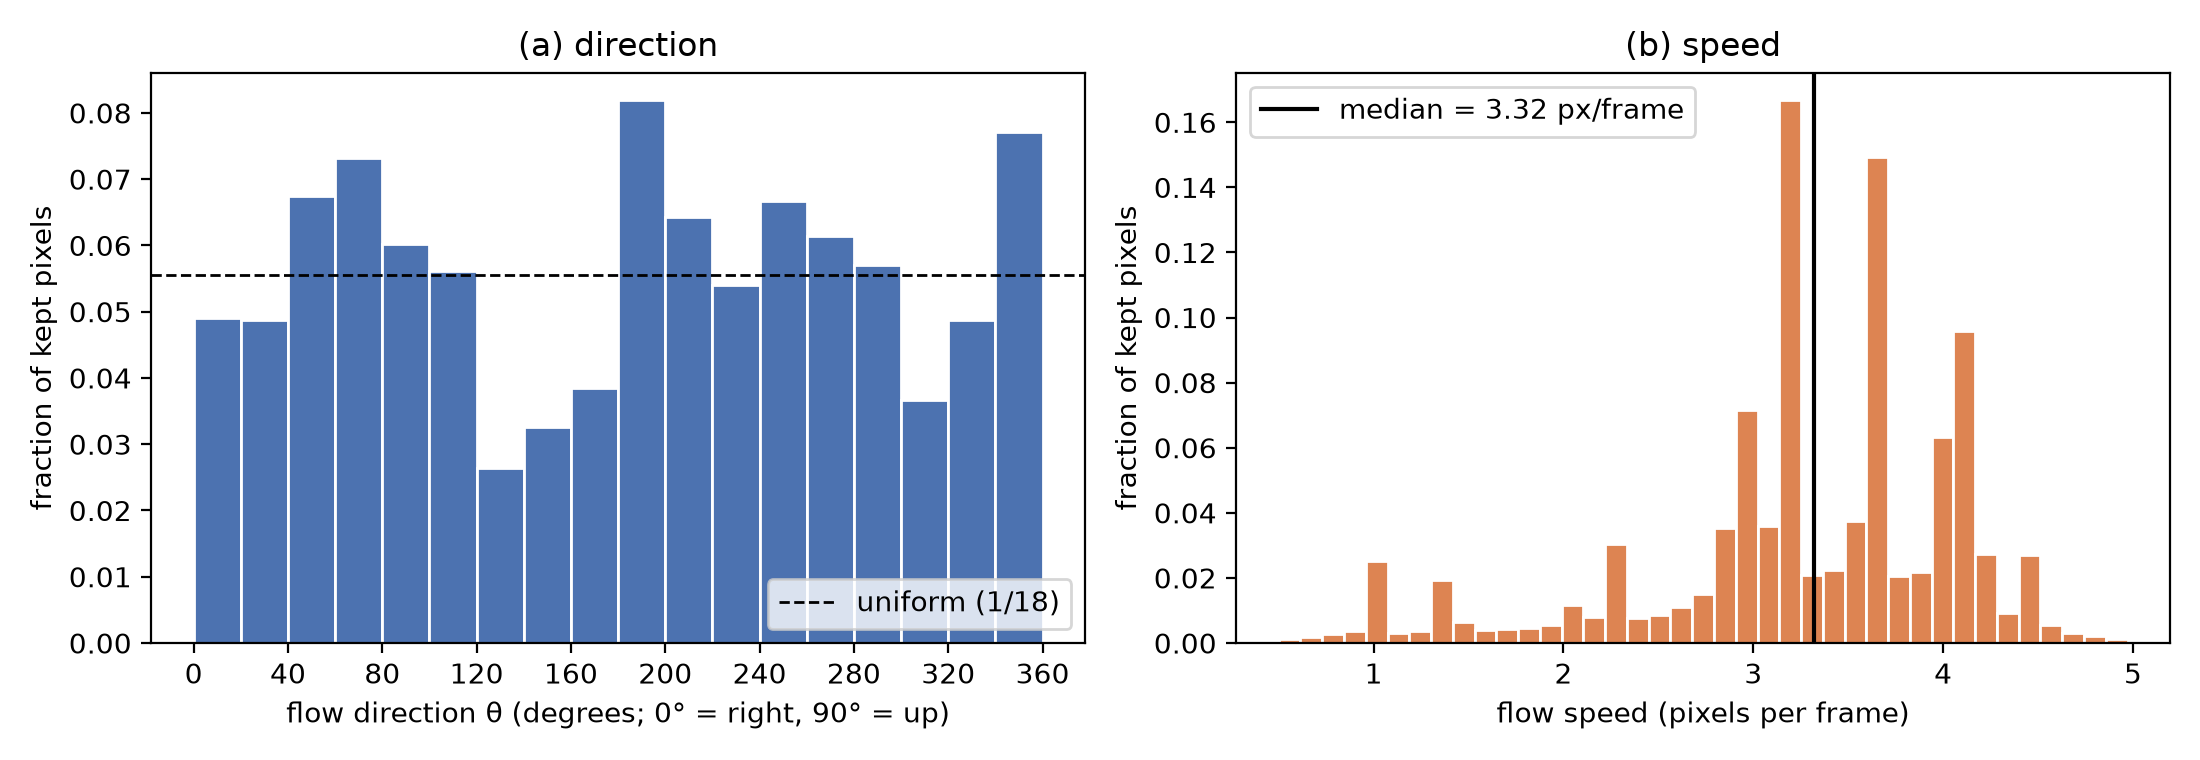
\includegraphics[width=\textwidth]{figure1.png}
  \caption{Optical flow on the first 50 training videos (950 frame pairs, Farneback). (a) Direction of motion, 18 bins of 20$^\circ$; the dashed line is a uniform spread (1/18). (b) Speed in pixels per frame. Both show the fraction of kept pixels. Median speed: 3.32 pixels per frame. Pixels kept: 103,050.}
\end{figure}

\textbf{Q2.1} Yes. Mirrored and rotated motion is already familiar. In Figure 1(a) every 20$^\circ$ direction holds between 2.6\% and 8.2\% of the moving pixels; no direction is missing. Mirroring turns a direction $\theta$ into $180^\circ - \theta$, and a 90$^\circ$ rotation turns it into $\theta + 90^\circ$. Both only reshuffle the bars of a histogram that already covers every direction, so a mirrored or rotated video moves in directions the model has seen many times. The bars are uneven only because 50 videos contain about 100 digits, and each digit keeps one direction between bounces. Figure 1(b) shows a typical speed of 3.32 pixels per frame (half of all pixels between 3.00 and 3.89). So 2$\times$ is about 6.6 and 3$\times$ about 10.0 pixels per frame, both faster than almost anything in training. Where digits overlap, the flow is wrong, which likely explains the small bumps near 1 pixel per frame. Overlaps are short and happen in all directions, so they add a little noise but cannot fill or empty a whole direction. The answer does not change.

\textbf{Q2.2} Mirror and rotation change only the \emph{appearance} of the digits; the motion statistics stay the same, because the direction histogram is already full (Q2.1) and the speed does not change. Rotation changes appearance more than mirroring. Speed-up does the opposite: it changes only the \emph{motion} (each step is $k$ times longer), while the digits look the same. So each test changes one thing and keeps the other fixed. If the model fails a mirror or rotation test, the cause is appearance. If it fails a speed test, the cause is motion. This is what makes them a controlled experiment.

% ---------------------------------------------------------------------
\subsection*{2. Baseline: ConvLSTM}

%Q2-BASELINE-RESULTS

\textbf{Q2.3} Model A's reach is \textbf{8 pixels per time step}. One cell of the folded $16\times16$ grid is 4 original pixels. Pixel-unshuffle, the $1\times1$ output convolution and pixel-shuffle do not move information. Only the two $3\times3$ convolutions do, and each moves it by at most one cell (4 pixels). Within one step $\tau$:
\begin{itemize}
  \item from the new input $u_\tau$: layer-1 convolution (1 cell) $\rightarrow h^{(1)}_\tau \rightarrow$ layer-2 convolution (1 cell) $\rightarrow h^{(2)}_\tau \rightarrow$ output: \textbf{2 cells};
  \item from $h^{(1)}_{\tau-1}$: it enters the same layer-1 convolution, so the path is also \textbf{2 cells};
  \item from $h^{(2)}_{\tau-1}$: only the layer-2 convolution, \textbf{1 cell};
  \item the cell states $c^{(\ell)}_{\tau-1}$ are only multiplied pixel by pixel, so they add no distance (at most the 1 cell of layer 2 for $c^{(1)}$).
\end{itemize}
The longest path is 2 cells $= 2 \times 4 = 8$ pixels. A digit that moves more than about 8 pixels between frames cannot be linked to its old position in a single update.

%Q2-4

\textbf{Q2.5} (written and committed before any experiment in Testing the Baseline; copied unedited from \texttt{Question2/predictions/Q2.5.md})

\begin{quote}\small
\textbf{Mirror test.} Figure 1(a) shows digits moving in every direction, so mirrored motion is motion model A has already seen. Only the look of the digits is new (a mirrored 2 is not a 2). I expect model A to mostly pass: the digits should still move the right way, but their shapes may blur or drift back towards normal-looking digits. So E\_M should be a little higher than E(5), and C\_M small but not zero.

\textbf{Rotation test.} The motion is again familiar, but rotated digits look even less like the training digits than mirrored ones. I expect model A to do worse than on the mirror test (C\_R $>$ C\_M and E\_R $>$ E\_M), while the digits still move in roughly the right direction.

\textbf{Speed.} The median speed is about 3.3 pixels per frame, so 2x is about 6.6 and 3x about 10 pixels per frame. Model A can move information at most 8 pixels per step. At 2x the motion is still inside this reach, but the model never saw such fast motion in training, so I expect some extra error but no breakdown. At 3x most motion is beyond the reach, so I expect model A to break down there: blurred digits that stay near their old position or fade away.
\end{quote}

%Q2-TESTING


% =====================================================================
\end{document}
